{\color{teal!90}\chapter{Change Log}\label{cap:change-log}}
  \AddToShipoutPictureBG*{%
    \AtPageUpperLeft{%
      \raisebox{-\height}{%
        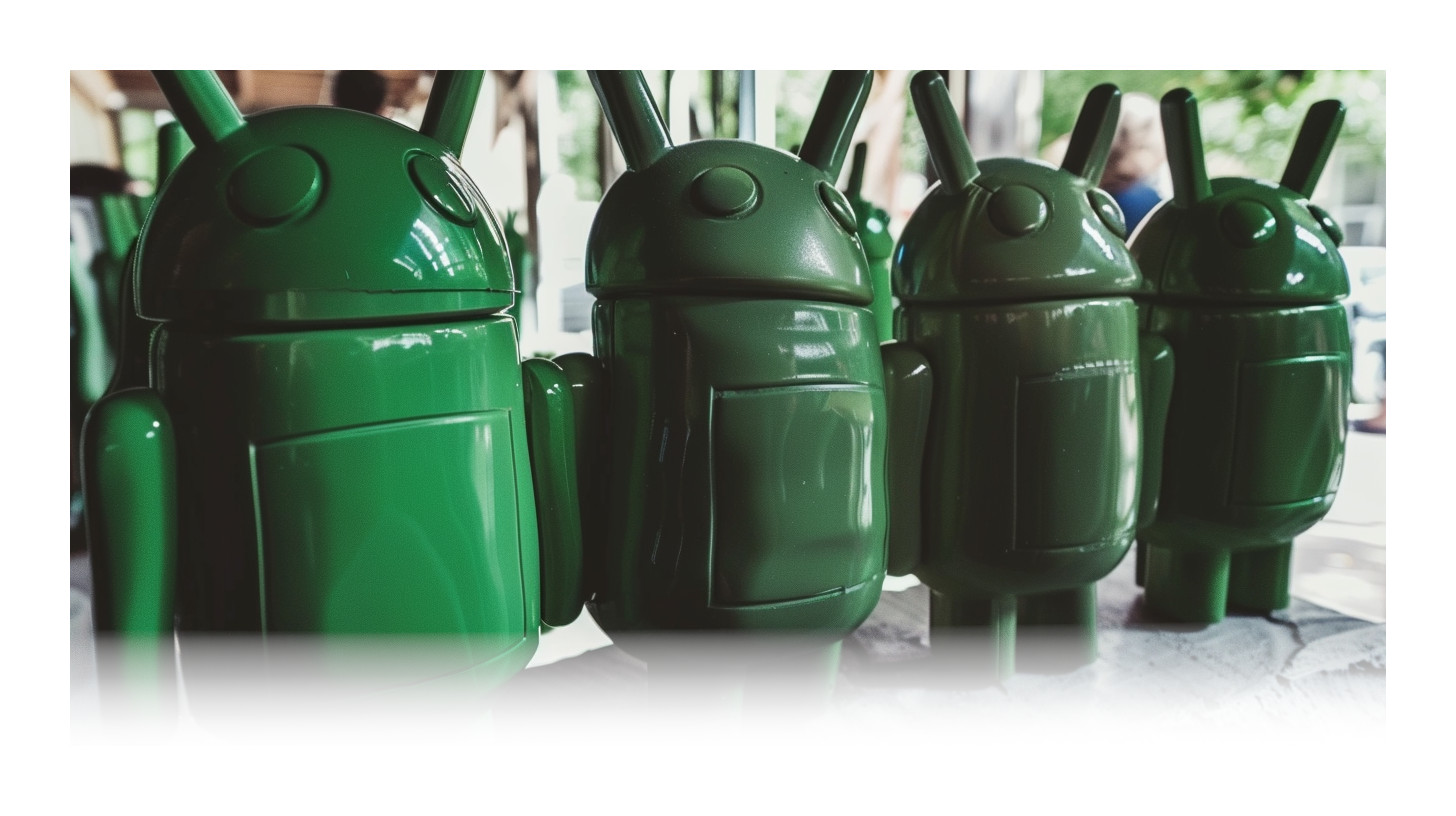
\includegraphics[width=\paperwidth]{./chapters/chapter-header-change-log.jpg}%
      }%
    }
  }

  \minitoc % Creating an actual minitoc mini lista contenuti

%  \section{Change Log}
%
%  \subsection{Firmware Change Log}

  \section{DWPS-13\_K04\_XMA311D2AV2-1\_A311D2\_8192M\_128G\_USBUART\_Airgo-0.0.0-20240611225217}
    \label{sec:firmware20240611225217}

  I had to disable com.xbh.share (AirgoCast v. \emph{\color{Grey}2.9.1.381.B}) to get the Wifi working. The firmware was periodically disconnecting every 2 minutes and 9 seconds\footnote{The disconnection frequency was calculated using the Python code in Listing\ref{lst:python-dhcp} and the accurate result is (2, 9.997571428571433)}. Figure \ref{fig:change-log} shows how frequent the disconnections were. The DhcpClient kept dropping down \textbf{onQuitting}.

  I went back to an even older firmware where the problem wasn't there but the screencasting app was super old.
  I removed the super old screencasting app. Installed com.xbh.share and the problem came back. I had to disable it again to get the Wifi working.
\clearpage
\lstinputlisting[language=Python, caption=Python code to calculate the disconnection frequency, label=lst:python-dhcp]{./chapters/change-log/dhcp-calc.py}

  \begin{figure}
    \centering
    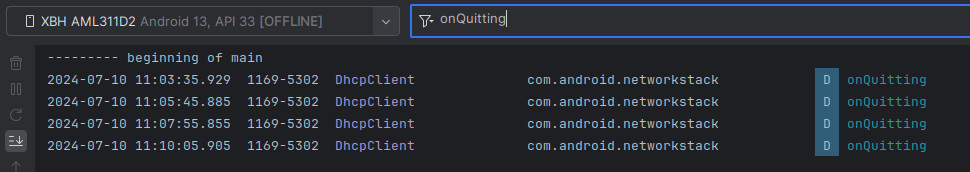
\includegraphics[width=0.9\textwidth]{./chapters/change-log/change-log.jpg}
    \caption{DHCP Client kept dropping down \textbf{onQuitting}}
    \label{fig:change-log}
  \end{figure}

  \section{DWPS-13\_K04\_XMA311D2AV2-1\_A311D2\_8192M\_128G\_USBUART\_Airgo-0.0.0-20240705151015}
    \label{sec:firmware20240705151015}

  The frequent disconnections is now fixed (AirgoCast v. \emph{\color{Grey}2.10.1.404.B}), but we noticed we couldn't see 2.4 Ghz signals easily.
  We had to manually determine the optimal Wi-Fi channel settings for the Akhter2\_4 network to ensure visibility and connectivity on the IFP.

  \begin{itemize}
    \item The router was set to the \textbf{Auto channel} mode.
    \item The Android IFP was able to detect and connect to the Akhter2\_4 network.
  \end{itemize}

  \paragraph{Testing on Channel 13}
  \begin{itemize}
    \item The router was manually set to \textbf{channel 13}.
    \item The Akhter2\_4 network became invisible on the Android device.
  \end{itemize}

  \paragraph{Reverting to Auto Channel}
  \begin{itemize}
    \item The router was reverted to \textbf{Auto channel} mode.
    \item Using the Net Analyzer app, it was determined that the router was operating on \textbf{channel 1}.
    \item With this setting, the Akhter2\_4 network was visible and accessible again on the Android device.
  \end{itemize}


  \paragraph{Channel 13 Visibility Issue}
  \begin{itemize}
    \item On 9th July 2024, having the router to channel 13\footnote{it's always been like this since my 1st day} allowed the Akhter2\_4 network to be visible and accessible on the Android device.
    \item On 10th July 2024, however, channel 13 prevents the Akhter2\_4 network from being seen by the Android device.
    \item This indicates a change in the network environment or interference on channel 13 that is now obstructing the visibility of Akhter2\_4.
  \end{itemize}

  \paragraph{Signal Strength Adjustment}
  \begin{itemize}
    \item Increasing the signal strength from medium to strong did not result in any improvement in the visibility of the Akhter2\_4 network on channel 13.
  \end{itemize}

  The tests indicate that while channel 13 was previously a viable option, it now poses an issue for network visibility on the Android device. The \textbf{Auto channel} setting, which defaults to \textbf{channel 1} in this environment, ensures that the Akhter2\_4 network remains visible and accessible. Signal strength adjustments did not mitigate the visibility issue on channel 13. Therefore, it is recommended to continue using the Auto channel setting to maintain reliable connectivity for the Akhter2\_4 network.

  \paragraph{Additional Tests}
  \begin{itemize}
    \item Channel 12: The WiFi is still not visible.
    \item Channel 11: The WiFi is visible.
  \end{itemize}

  There's a bug where the touch screen freezes on both firmwares (page \pageref{sec:firmware20240611225217} and page \pageref{sec:firmware20240705151015}).

  \paragraph{Channel Visibility Tests}
  \begin{itemize}
    \item Channel 10: Akhter2\_4 is visible on the unlocked screen close to production door with strong signal.
    \item Channel 9: Akhter2\_4 is visible on the unlocked screen close to production door but with weak signal. Visible on the locked-down screen in my corner.
    \item Channel 8: Akhter2\_4 is visible on the unlocked screen close to production door but with weak signal. Visible on the locked-down screen in my corner.
    \item Channel 7: Akhter2\_4 is visible on the unlocked screen close to production door but with weak signal. Visible on the locked-down screen in my corner.
    \item Channel 6: Akhter2\_4 is visible on the unlocked screen close to production door but with weak signal. Visible on the locked-down screen in my corner.
    \item Channel 5: Akhter2\_4 is visible on the unlocked screen close to production door but with weak signal. Visible on the locked-down screen in my corner.
    \item Channel 4: Akhter2\_4 is visible on the unlocked screen close to production door but with weak signal. Visible on the locked-down screen in my corner.
    \item Channel 3: Akhter2\_4 is visible on the unlocked screen close to production door but with weak signal. Visible on the locked-down screen in my corner.
    \item Channel 2: Akhter2\_4 is not visible on the unlocked screen close to production door. Visible on the locked-down screen in my corner but with one bar less.
    \item Channel 1: Akhter2\_4 has very weak signal on the unlocked screen close to production door and sometimes disappears. Very strong on the locked-down screen in my corner.
    \item Channel 13: Akhter2\_4 is not visible on the unlocked screen close to production door. Not visible on the locked-down screen in my corner.
  \end{itemize}

  At 11:53 on 10th July 2024 the Android IFP touch running the firmware shown on page \pageref{sec:firmware20240611225217} froze.
  At 12:36, we returned to Auto which is on channel 1. Akhter2\_4 is strongly visible on the unlocked screen close to production door and very weak and disappearing on the locked-down screen in my corner.

  At 12:09, I interacted with the screen with Touch frozen.
  At 12:22, I retouched the screen unlocked with log running.

  On 12th July at 11:39 the firmware shown on page \pageref{sec:firmware20240705151015} had the same old Wifi issue commented out in the video I've sent to Slin.
  The WiFi just stops connecting even to open Wifi. The only way to fix it is to restart the device.

  We have also noticed the Log doesn't create the folder when the log starts

  None of these problems are occurring with 5 GHz networks. All 16 channels have been tested and the results are consistent.
